% Search for all the places that say "PUT SOMETHING HERE".

\documentclass[11pt]{article}
\usepackage{amsmath,textcomp,amssymb,graphicx,enumerate,hyperref,enumitem,mathtools,tikz-qtree,listings,tikz}

\def\Name{Jonathan Sun}  % Your name
\def\SID{25020651}  % Your student ID number
\def\Homework{2} % Number of Homework
\def\Session{Fall 2017}


\title{CS170 --- \Session --- Homework \Homework \space Solutions}
\author{\Name, SID \SID}
\markboth{CS170 --- \Session --- Homework \Homework \space --- \Name}{CS170 --- \Session --- Homework \Homework --- \Name}
\pagestyle{myheadings}
\date{}

\def\endproofmark{$\Box$}
\newenvironment{proof}{\par{\bf Proof:}}{\endproofmark\smallskip}
\newenvironment{FourPartSolution}{\par{\bf Four-Part Solution:}}{\smallskip}
\newenvironment{mainIdea}{\par{\bf Main Idea:}}{\smallskip}
\newenvironment{pseudocode}{\par{\bf Pseudocode:}}{\smallskip}
\newenvironment{proofOfCorrectness}{\par{\bf Proof of Correctness:}}{\endproofmark\smallskip}
\newenvironment{runTime}{\par{\bf Run Time:}}{\smallskip}
\newenvironment{justification}{\par{\bf Justification:}}{\smallskip}
% \newenvironment{proofOfCorrectness}{\par{\bf Proof of Correctness:}}{\endproofmark\smallskip}
% \newenvironment{runTime}{\par{\bf Run Time:}}{\smallskip}
% \newenvironment{justification}{\par{\bf Justification:}}{\smallskip}

\usepackage[margin=1in]{geometry}



\begin{document}
\maketitle

Collaborators: Kevin Vo, Aleem Zaki, Jeremy Ou

\section*{1. Minimal Positive Valued Function}
\begin{FourPartSolution}
\begin{mainIdea}
\\
We are going to take advantage of the idea of that the output of $f(i)$ will always be greater than the output of $f(i + 1)$. This means that as we test greater and greater inputs, we will approach a negative output more and more closely. Since the function only takes natural numbers as input, we first try $f(1)$ as the first possible input. If $f(1) < 0$, we have our answer. Otherwise, I will test inputs (starting with $2$) that I repeatedly square until $f(i) < 0$. When I reach this point, I will know that $n$ is $\sqrt{i} < n < i$.
\end{mainIdea}
\\
\begin{pseudocode}
\begin{lstlisting}
# findRangeOfN will find what the sqrt(i) and i are
# in which sqrt(i) < n < i is true
findRangeOfN(f(x)):
	# testing it with the first natural number (which is 1)
	# if f(1) is negative, then we know that n = 1
	# is the smallest n where the output of f(i) is negative
	if f(1) < 0:
		return 1
	# i = 2 is the next natural number
	i = 2
	# when f(i) is negative we will exit the loop
	# otherwise square i repeatedly until we find f(i) is negative
	# oldI is the i that is passed into each iteration of the loop
	while f(i) >= 0:
		oldI = i
		i = i^2
	# use the helper function which will return the correct n
	# pass in the f(x), oldI = sqrt(i), and i
	return helper(f(x), oldI, i)

# helper function will return the integer n
helper(f(x), oldI, i):
	# take the middle integer between sqrt(i) and i
	# floor division to ensure that it is an integer
	newI = (oldI + i) // 2
	# base case where we return the integer n that satisfies f(i) < 0
	if f(newI) >= 0 and f(newI + 1) < 0:
		return newI + 1
	# recursive call between newI and i since
	# we know that n is greater than newI
	if f(newI) > 0:
		return helper(f(x), newI, i)
	# recursive call between oldI and newI since
	# we know that n is less than newI
	else:
		return helper(f(x), oldI, newI)
\end{lstlisting}
\end{pseudocode}
\begin{proofOfCorrectness}
\\
Because the function is strictly decreasing, this means that as $i$ increases, the function will approach $0$ and then become negative. So my strategy is to start from the smallest natural number as the input $i$ and increase $i$ if needed to find the mininum natural number $i$ that gives $f(i) < 0$.
\vspace*{1\baselineskip}
\\
The first natural number is $1$ so I first try $f(1)$ and if $f(1) < 0$ then I will know that $1$ is the smallest natural number input for $f(i)$ where the function becomes negative. Otherwise, I continue by setting $i = 2$ and testing if $f(2) < 0$ and repeatedly square $i$ until I find an $i$ that is negative. Because I am repeatedly squaring $i$, this takes $O(\log{n})$ time. This means that the input $i$ before that is $\sqrt{i}$ and so the answer is between $\sqrt{i}$ and $i$. To find the answer I pass the function, $\sqrt{i}$ as $oldI$, and $i$ into a helper function which will solve for the answer.
\vspace*{1\baselineskip}
\\
For this helper function that solves for the actual answer, I first find the average natural number between $\sqrt{i}$ and $i$ with $newI = (oldI + i) // 2$ where $newI$ is the average natural number. I then check for if $f(newI) >= 0$ and $f(newI + 1) < 0$. If this is true, then I know that the smallest natural number input into the function that gives a negative result is $newI + 1$. If $f(newI) > 0$, then I can do a recursive call on the helper function with the search space being between $newI$ and $i$. If $f(newI) < 0$, then I can do a recursive call on the helper function with the search space being between $oldI$ and $newI$. Since both recursive calls reduces the search space by halving the previous search space, the two recursive calls have $O(\log{n})$ time. 
\end{proofOfCorrectness}
\\
\begin{runTime}
\\
$O(\log{n})$.
\end{runTime}
\\
\begin{justification}
\\
My main function, which is $findRangeOfN(f(x))$, has a while loop that repeatedly squares $i$ as opposed to increasing $i$ at a constant pace. Therefore, getting the range where the answer lies, which is between $\sqrt{i}$ and $i$, takes $O(\log{n})$ time. My helper function also runs in $O(\log{n})$ time because my recursive calls decrease the search space to find the answer by halving the search space during every recursive call. Therefore, the run time is $O(\log{n} + \log{n}) = O(2\log{n}) \approx O(\log{n})$.
\end{justification}
\end{FourPartSolution}



\newpage
\section*{2. Graph Basics}
\begin{enumerate}[label=(\alph*)]
\item
A, B, D, E, G, F, C, H, I.
\vspace*{1\baselineskip}
\\
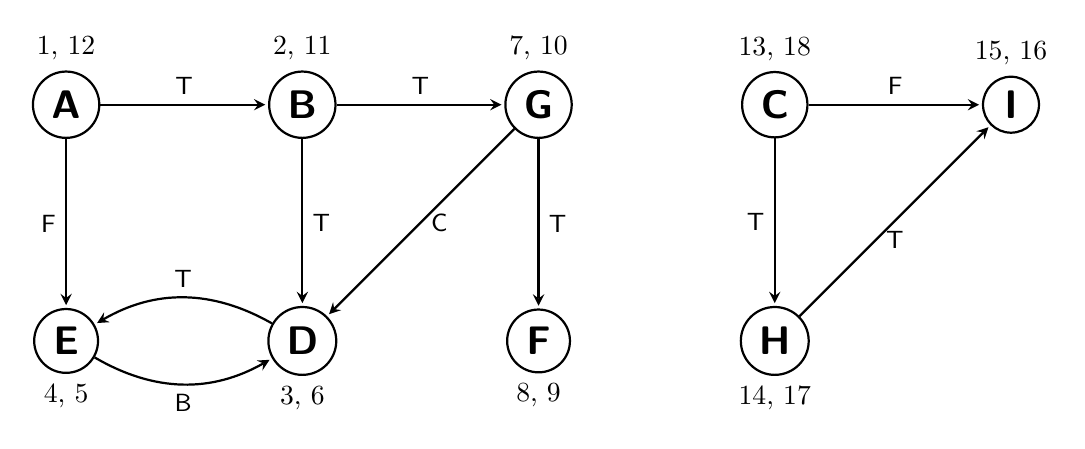
\begin{tikzpicture}[->, >=stealth, shorten >=1pt, auto, node distance=3cm, thick, main node/.style={circle, draw, font=\sffamily\Large\bfseries}]
	\node[main node, label=above:$1\text{, }12$] (A) {A};
	\node[main node, label=above:$2\text{, }11$] (B) [right of=A] {B};
	\node[main node, label=above:$7\text{, }10$] (G) [right of=B] {G};
	\node[main node, label=below:$4\text{, }5$] (E) [below of=A] {E};
	\node[main node, label=below:$3\text{, }6$] (D) [below of=B] {D};
	\node[main node, label=below:$8\text{, }9$] (F) [below of=G] {F};
	\node[main node, label=above:$13\text{, }18$] (C) [right of=G] {C};
	\node[main node, label=above:$15\text{, }16$] (I) [right of=C] {I};
	\node[main node, label=below:$14\text{, }17$] (H) [below of=C] {H};

	\path[every node/.style={font=\sffamily\small}]
		(A) edge node [above] {T} (B)
			edge node [left] {F} (E)
		(B) edge node [right] {T} (D)
			edge node [above] {T} (G)
		(G) edge node [right] {C} (D)
			edge node [right] {T} (F)
		(D) edge [bend right] node [above] {T} (E)
		(E) edge [bend right] node [below] {B} (D)
		(C) edge node [left] {T} (H)
		(C) edge node [above] {F} (I)
		(H) edge node [below] {T} (I);
\end{tikzpicture}

\item
A simple graph is a graph that has no parallel edges or self-loops. This means that a graph with just one node will have no edges since it cannot have an edge with itsself. When considering a graph with just two nodes, there can only be one edge since there is an edge that can be drawn from the first node to the second node but there cannot be a parallel edge drawn from the second node back to the first node. When considering a graph with just three nodes, the first node can have two edges drawn (one edge connects to the second node and one to the third node), the second node can have one edge drawn (that edge connects the second node to the third node), and the third node has no edges that can be drawn since this is a simple graph. This gives it a total of three edges. With this, I have noticed that the number of edges in a simple graph can be represented as $(|V| - 1) + (|V| - 2) + ... + 3 + 2 + 1$ or alternatively:
\begin{align*}
\sum\limits_{i = 1}^{|V| - 1} i = 1 + 2 + 3 + ... + (|V| - 1) = ((|V| - 1) + 1)\frac{|V| - 1} {2} = \frac{|V| (|V| - 1)} {2} \in O(|V|^2)
\end{align*}

\item
For $\sum d_i$ to be even, it must be able to be modeled as $2k$ where k is an integer. To prove this, I will start with a case where there is no existing edge, which is an even degree of edges. When I add an edge, the degree of the edges increases by $2$ because an edge always connects $2$ vertices which means that both vertix increases by degree $1$ each. This means that whenever an edge is added, the degree of the edges increases by $2$ each time. So, if you add $k$ edges, then the degree of the edges increases by $2k$. This is even by the definition as I provided in the first sentence.

\end{enumerate}



\newpage
\section*{3. Peak Element}
\begin{FourPartSolution}
\begin{mainIdea}
\\
The main idea of the question is that we need to just need to find one peak even if there can exist multiple peaks. To do so, I will try to split the search space in half when recursing through the array of houses by comparing the middle indexed house with its neighbors and searching the side which has the larger neighbor if the middle indexed house is not already a peak.
\end{mainIdea}
\\
\begin{pseudocode}
\begin{lstlisting}
# inputArray is of length n
findPeak(inputArray[...]):
	# get the middle index (integer) of the search space
	mid = n // 2
	# if inputArray[mid] is a peak then return the middle index
	if inputArray[mid - 1] < inputArray[mid] < inputArray[mid + 1]:
		return mid
	# if value on the left of the middle index is greater
	# then there exists a peak in the left half of inputArray
	# recursive call on the left half of inputArray
	else if inputArray[mid - 1] > inputArray[mid]:
		return findPeak(inputArray[0 : (mid - 1)])
	# if value on the right of the middle index is greater
	# then there exists a peak in the right half of inputArray
	# recursive call on the right half of inputArray
	# add m to get the proper index since m changes when recursing
	else:
		return findPeak(inputArray[(mid + 1) : n]) + mid
\end{lstlisting}
\end{pseudocode}
\begin{proofOfCorrectness}
\\
For a house to have a view, that house must be taller than the houses next to it. This also means that if the current house you are looking at is shorter than a house to its right, then it is guaranteed that there exists a house somewhere to the right of the current house which is a peak. This is true because the peak can be the house directly to the right all the way to the end of the street. Since we know that there is a peak somewhere to the right of the current house, we can recursively search for the peak by reducing the search size of the array of houses by $\frac{1} {2}$ each time. We can apply the same concept to the houses on the left of the current house if the house to the left of the current house is taller. Regardless, whenever we recurse, we are decreasing the search space by $\frac{1} {2}$ each time.
\end{proofOfCorrectness}
\\
\begin{runTime}
\\
$O(\log{n})$.
\end{runTime}
\\
\begin{justification}
\\
The run time is $O(\log{n})$ because each recursive call halves the size of the search space. Therefore, the run time is $O(\log{n} + \text{constant work to compare}) \approx O(\log{n})$.
\end{justification}
\end{FourPartSolution}



\newpage
\section*{4. Exact Change}
\begin{FourPartSolution}
\begin{mainIdea}
\\
The main idea is that there is only $4$ of each type of coin and that we need to use exactly $4$ coins but to find all the possible sums of $4$ of each type of coin we can take advantage of the properties of exponents in polynomials. First, you need to set up the polynomial in the following format:
\begin{align*}
a(x) = x^{A[0]} + x^{A[1]} + ... + x^{A[n - 1]}
\end{align*}
The property of exponents in polynomials is that when multiplying $2$ polynomials together, you can add the exponents together. For example, $x^2 * x^3 = x^{2 + 3} = x^5$. Using this idea, if I can find a polynomial with the exponent equal $t$ then it is possible to give the exact change using exactly $4$ coins. This can be done by doing the Fast Fourier Transformation twice.
\end{mainIdea}
\\
\begin{pseudocode}
\\
define: $a(x) = x^{A[0]} + x^{A[1]} + ... + x^{A[n - 1]}$
\begin{lstlisting}
exactChange(A[0, 1, ..., n - 1], t):
	# polynomial and exponents of twoCoins will
	# give all possible combinations of two coins
	# calculation done with Fast Fourier Transformation
	twoCoins = (a(x))(a(x))
	# polynomial and exponents of fourCoins will
	# give all possible combinations of four coins
	# calculation done with Fast Fourier Transformation
	fourCoins = (twoCoins)(twoCoins)
	# return if coefficient of x^t is greater than 0
	# return false if no coefficient exists for x^t
	if (coefficient of x^t) != 0:
		return true
	return false
\end{lstlisting}
\end{pseudocode}
\begin{proofOfCorrectness}
\\
In my pseudocode, I relied on Fast Fourier Transformation twice to find if a coefficient exists for $x^t$. My logic behind this is that when I multiply $a(x)$ with $a(x)$ by using Fast Fourier Transformation, I end up getting a polynomial that is of degree $2A[0]$ and that the exponents in each polynomial represent all the possible combinations if the problem stated that we needed to use exactly $2$ coins. By squaring this again using Fast Fourier Transformation again, I get a polynomial with each exponent representing the all possible values that one can get using exactly $4$ coins. Basically, by matching each term of $a(x)$ with each term of $a(x)$ with each term of $a(x)$ with each term of $a(x)$, we get all possible quartet combinations with $4$ coins. If the coefficient exists for $x^t$ that is not zero, then you know that a combination of $4$ coins exist where the value of the $4$ coins is $t$.
\end{proofOfCorrectness}
\\
\begin{runTime}
\\
$O(n\log{n})$.
\end{runTime}
\\
\begin{justification}
\\
The justification for the $O(n\log{n})$ run time is that the first Fast Fourier Transformation takes $O(n\log{n})$ time. Since our polynomial is doubled in length for the second Fast Fourier Transformation, it takes $O(2n\log{2n})$ to do the second Fast Fourier Transformation. Last, the $4n + 1$ come from the fact that you must find if a nonzero coefficient exists for $x^t$ by checking up to $4n + 1$ values. This gets the run time to be $O(n\log{n} + 2n\log{2n} + 4n + 1) \approx O(n\log{n})$ and $O(n\log{n})$ is faster than $O(n^2)$.
\end{justification}
\end{FourPartSolution}



\newpage
\section*{5. Local Maxima}
\begin{FourPartSolution}
\begin{mainIdea}
\\
The main idea of this is that we alternate using peak element on the columns and rows of the matrix. This works because there exists only one local maximum in each column and only one in the entire matrix. This ensures that by using peak element, we will only get the local maximum in the since we can only get the local maximum in each column and in each row. This means that we will divide and conquer the search space in half each time we run the peak element strategy when alternating between columns and rows.
\end{mainIdea}
\\
\begin{pseudocode}
\\
\begin{lstlisting}
LocalMaxima(Matrix n):
	if maxima in findPeak(middleColumn - 1) < maxima
	 in findPeak(middleColumn) < maxima
	 in findPeak(middleColumn + 1):

		if maxima in findPeak(middleRow - 1) < maxima
		 in findPeak(middleRow) < maxima
		 in findPeak(middleRow + 1):
			return maxima
		else if maxima in findPeak(middleRow - 1) > maxima
		 in findPeak(middleRow):
			return localMaxima(top half of Matrix n)
		else:
			return localMaxima(bottom half of Matrix n)
	else if maxima in findPeak(middleColumn - 1) > maxima
	 in findPeak(middleColumn):
		return localMaxima(left half of Matrix n)
	else:
		return localMaxima(right half of Matrix n)

# peak element pseudocode from above
findPeak(inputArray[...]):
	mid = n // 2
	if inputArray[mid - 1] < inputArray[mid] < inputArray[mid + 1]:
		return mid
	else if inputArray[mid - 1] > inputArray[mid]:
		return findPeak(inputArray[0 : (mid - 1)])
	else:
		return findPeak(inputArray[(mid + 1) : n]) + mid
\end{lstlisting}
\end{pseudocode}
\begin{proofOfCorrectness}
\\
The proof of this is that for every time I call the peak element on a column or row, I must call peak element on the array of that column or row recursively. This will guarantee to give me the local maxima of the matrix since there cannot be two local maximas in the entire matrix, as stated in the problem. This can be proved with proof by contradiction. Our algorithm will always return the local maximum between itself and its neighbors. So, if there is a local maxima on one side, but our algorithm takes us to the other side, then this contradicts the problem because there can only be one local maxima in the entire matrix.
\end{proofOfCorrectness}
\\
\begin{runTime}
\\
$O((\log{n})^2)$
\end{runTime}
\\
\begin{justification}
\\
The justification of this is that I will be halving the search space each time I find the peak element of a column or row in the matrix. This gives me $O(\log{n})$ run time. However, for every time I run peak element on a column or row in the matrix, I must also run it on the array in that column or row, which is also $O(\log{n})$. Therefore, the total run time is that I must run peak element for every peak element recursively so it becomes $O((\log{n})(\log{n})) = O((\log{n})^2)$.
\end{justification}
\end{FourPartSolution}



\newpage
\section*{6. DNA Sequence Alignment}
\begin{enumerate}[label=(\alph*)]
\item
\begin{pseudocode}
\begin{lstlisting}
# brute force algorithm that takes in s and t as binary strings
# where s is m bits long and t is n bits long
bruteForce(s, t, m, n, k):
	answer = []
	i = 0
	while i < n:
		j = 0
		copyOfi = i
		errors = 0
		while j < m:
			if s_j = t_copyOfi:
				if j = m - 1:
					answer.append(i)
				j++
				copyOfi++
			else:
				errors++
				if errors > k:
					break
		i++
	return answer
\end{lstlisting}
\end{pseudocode}

\item
The strategy of this is to take advantage of the fact that in binary, there are only $1$s and $0$s. To ensure that when multiplying polynomials $p(x)$ and $q(x)$ with FFT I can still find out if there are matches ($1$ matches with $1$ and $0$ matches with $0$), I change the $0$s to $-1$ so that when a $0$ matches with a $0$, this gives me $-1 * -1 = 1$. By using this strategy, I will know when FFT gives me polynomials with exponents being $1$s if they match or $0$s if there are no matches, which is the equivalent to whether a bit in $s$ matches that of $t$. Once I get a polynomial, I get the coefficients of the parts of the polynomial that are with exponent of $m - 1 + i$, as stated in the problem. I compare the coefficient with $m - 2k$ and if the coefficient between $m - 2k$ and $m$, then we have found a solution.

\item
When solving for $p(x)q(x)$ using FFT, we search for if there exists a part of the polynomial where the coefficient is between $m - 2k$ and $m$. If this coefficient does not exist, then we know that $s$ is not a substring of $t$ with $k$ errors. Otherwise, because the coefficients are equivalent to the number of matches with consideration to the $k$ errors we are allowed to have, we can recover what the $i$ is since we know that the coefficient is valid so we get the index $i$ from setting the exponent of that valid part of the polynomial to equal $m - 1 + i$. THis will take $O(n\log{n})$ time since the cost of calculating $p(x)q(x)$ using FFT takes $n - 1 + m + 1$ time. Overall the run time comes out to be $O((n + m - 2)\log{(n + m - 2)}) \approx O(n\log{n})$.

\item
The idea is to let $A = 0001$, $C = 1001$, $G = 0111$, and $T = 1111$ since we know that we get a match if the four rightmost bits gives us $0001$. For example, squaring any of those binary values and taking the four rightmost bits of them gives us $0001$ but multiplying $A$ with $C$ will gives us $1001$ as the four rightmost bits, which is not $0001$. With this modification, we can once check to see if we have a coefficient that falls in between m-2k and m, and if that coefficient is valid, then find $i$ from the exponent of that part of the polynomial. The runtime is $O(n\log{n})$ and the justification is the same as that of part (c).

\item
Mandatory Extra Credit: This problem was beautiful and painful to do. :(

\end{enumerate}

\end{document}
